\section{Overview}\label{overview}

\begin{frame}{Context}

\begin{itemize}
\itemsep1pt\parskip0pt\parsep0pt
\item
  Joined SBA-Research in Janurary to help with an ongoing Internet-wide
  scanning project
\item
  We've conducted scans on e-mail related ports over the last couple of
  months
\item
  Currently digging through collected data and writing papers
\end{itemize}

\end{frame}

\begin{frame}{Targets and Methods}

\begin{itemize}
\itemsep1pt\parskip0pt\parsep0pt
\item
  SMTP(S), POP3(S), IMAP(S) and Legacy Ports
\item
  \texttt{masscan} and \texttt{sslyze} with a queueing framework built
  around it
\item
  Delay between handshakes in \texttt{sslyze} added

  \begin{itemize}
  \itemsep1pt\parskip0pt\parsep0pt
  \item
    some POP/IMAP daemons are easily DoSed
  \end{itemize}
\item
  Runs spanning months (roughly from April to June)
\item
  About 9.2 billon TLS handshakes with \texttt{sslyze}
\item
  Multiple \texttt{masscan} runs for banners/certs
\item
  triggered \texttt{dovecot} bug (CVE-2015-3420) :)

  \begin{itemize}
  \itemsep1pt\parskip0pt\parsep0pt
  \item
    initially discovered and investigated/reported upstream by Hanno
    Boeck
  \end{itemize}
\end{itemize}

\end{frame}

\section{Results}\label{results}

\begin{frame}{Protocol Support}

\begin{figure}[h!]
  \centering
  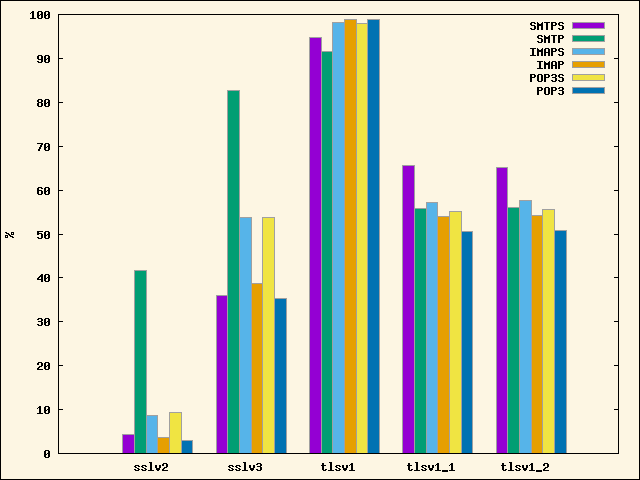
\includegraphics[scale=0.55]{protocol_support}
\end{figure}

\end{frame}

\begin{frame}{RC4}

\begin{table}[h]
\centering
\begin{tabular}{|l|rr|}
\hline
& Accepting RC4 & Not accepting RC4 \\
\hline
SMTPS & 82,27                & 17,73     \\
SMTP  & 86,27                & 13,73     \\
IMAPS & 83,36                & 16,64     \\
IMAP  & 85,71                & 14,29     \\
POP3S & 83,74                & 16,26     \\
POP3  & 86,51                & 13,49     \\
\hline
\end{tabular}
\caption{RC4 Cipher Support Percentage}
\label{tab:rc4-support-percentage}
\end{table}

\end{frame}

\begin{frame}{AUTH PLAIN offered by hosts}

\begin{block}{SMTP (25)}

\begin{itemize}
\itemsep1pt\parskip0pt\parsep0pt
\item
  917,536 - AUTH PLAIN, no STARTTLS support
\item
  1,722,387 - AUTH PLAIN \& STARTTLS
\end{itemize}

\end{block}

\begin{block}{IMAP (143)}

\begin{itemize}
\itemsep1pt\parskip0pt\parsep0pt
\item
  211,962 - AUTH PLAIN, no STARTTLS support
\item
  3,243,632 - AUTH PLAIN \& STARTTLS
\end{itemize}

\end{block}

\begin{block}{POP3 (110)}

\begin{itemize}
\itemsep1pt\parskip0pt\parsep0pt
\item
  225,341 - AUTH PLAIN, no STARTTLS support
\item
  3,391,525 AUTH PLAIN \& STARTTLS
\end{itemize}

\end{block}

\end{frame}

\begin{frame}{Certificates}

\begin{figure}[h!]
\centering
  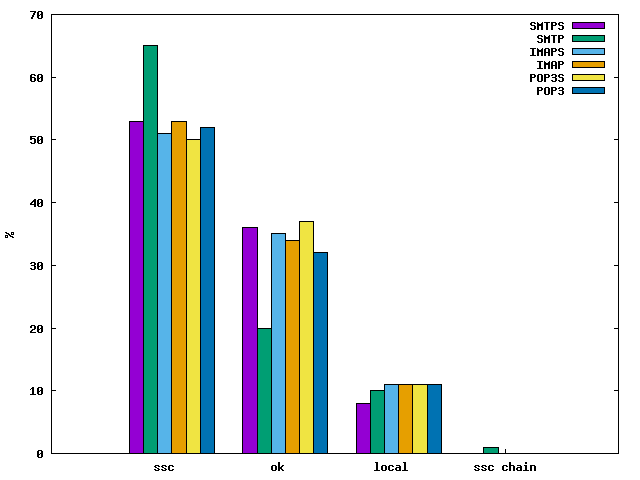
\includegraphics[scale=0.40]{pki}
\end{figure}

ssc: signed certificate, ok: CA signed, local: unable to get local
issuer certificate, ssc chain: self signed certificate in certificate
chain (Mozilla Truststore)

\end{frame}

\begin{frame}{Certificates (cont.)}

\begin{block}{SMTP and SMTPS}

\begin{itemize}
\itemsep1pt\parskip0pt\parsep0pt
\item
  Almost all leafs \textgreater{}= 1024 bit RSA (most 2048)
\item
  Same for intermediates (fewer than 200 with less than 1024 bit RSA)
\end{itemize}

\end{block}

\begin{block}{POP3(S) and IMAP(S)}

\begin{itemize}
\itemsep1pt\parskip0pt\parsep0pt
\item
  Very similar results, a few more low-bit leaf and intermediates.
\end{itemize}

\end{block}

\end{frame}

\begin{frame}{Weak ciphers and Anon-DH}

\begin{block}{SMTP (STARTTLS)}

\begin{itemize}
\itemsep1pt\parskip0pt\parsep0pt
\item
  RC2-CBC-MD5 - 40.9\% accept (26.5\% prefer!)
\item
  IDEA-CBC-MD5 - 14.4\% accept
\end{itemize}

\end{block}

\begin{block}{SMTPS}

\begin{itemize}
\itemsep1pt\parskip0pt\parsep0pt
\item
  Anon-DH suites: about 12\% acceptance
\end{itemize}

\end{block}

\begin{block}{POP(S)/IMAP(S)}

\begin{itemize}
\itemsep1pt\parskip0pt\parsep0pt
\item
  Nothing too exciting, ask me about details if you're interested
\end{itemize}

\end{block}

\end{frame}

\begin{frame}{Key-exchange}

\begin{block}{DH(E)}

\begin{itemize}
\itemsep1pt\parskip0pt\parsep0pt
\item
  Large number of 512bit DH primes in SMTP
\item
  Sigificant amount of DH group size =\textless{} 1024 in all studied
  protocols
\end{itemize}

\end{block}

\begin{block}{ECDH(E)}

\begin{itemize}
\itemsep1pt\parskip0pt\parsep0pt
\item
  Group size: most use 256, some 384, very few 521 throughout studied
  protocols
\end{itemize}

\end{block}

\begin{block}{Common Primes}

\begin{itemize}
\itemsep1pt\parskip0pt\parsep0pt
\item
  Apache prime (Adrian et al `Weak-DH' paper) not used
\item
  mod\_ssl prime: some users, very few
\end{itemize}

\emph{more on this topic TBD}

\end{block}

\end{frame}

\begin{frame}{Weak Keys}

Analyzed 40,268,806 collected certificates. Rather unspecacular:

\begin{block}{Fast-GCD (Heninger et al. ``Mining P's \& Q's'', algo. by
djb)}

\begin{itemize}
\itemsep1pt\parskip0pt\parsep0pt
\item
  30,757,242 RSA moduli
\item
  2,354,090 uniques
\item
  456 GCDs found
\end{itemize}

\end{block}

\begin{block}{Debian Weak-Keys (CVE-2008-0166)}

\begin{itemize}
\itemsep1pt\parskip0pt\parsep0pt
\item
  Compared to \texttt{openssl-blacklist} package
\item
  A single (1) match
\end{itemize}

\end{block}

\end{frame}

\section{Conclusion}\label{conclusion}

\begin{frame}{Conclusion}

\begin{itemize}
\itemsep1pt\parskip0pt\parsep0pt
\item
  First to conduct such a detailed study for E-Mail

  \begin{itemize}
  \itemsep1pt\parskip0pt\parsep0pt
  \item
    A lot of issues with transport security in the e-mail ecosystem
  \item
    Results are pretty much what we've expected beforehand
  \item
    We'll publish all collected datasets (soon-ish)
  \end{itemize}
\item
  More studies, analysis and papers forthcoming
\item
  We have tons of additional data, if you have specific questions write
  us!
\end{itemize}

\end{frame}
